%%%%%%%%%%%%%%%%%%%%%%%%%%%%%%%%%%%%%%%%%
% University Assignment Title Page 
% LaTeX Template
% Version 1.0 (27/12/12)
%
% This template has been downloaded from:
% http://www.LaTeXTemplates.com
%
% Original author:
% WikiBooks (http://en.wikibooks.org/wiki/LaTeX/Title_Creation)
%
% License:
% CC BY-NC-SA 3.0 (http://creativecommons.org/licenses/by-nc-sa/3.0/)
% 
% Instructions for using this template:
% This title page is capable of being compiled as is. This is not useful for 
% including it in another document. To do this, you have two options: 
%
% 1) Copy/paste everything between \begin{document} and \end{document} 
% starting at \begin{titlepage} and paste this into another LaTeX file where you 
% want your title page.
% OR
% 2) Remove everything outside the \begin{titlepage} and \end{titlepage} and 
% move this file to the same directory as the LaTeX file you wish to add it to. 
% Then add \input{./title_page_1.tex} to your LaTeX file where you want your
% title page.
%
%%%%%%%%%%%%%%%%%%%%%%%%%%%%%%%%%%%%%%%%%
%\title{Title page with logo}
%----------------------------------------------------------------------------------------
%	PACKAGES AND OTHER DOCUMENT CONFIGURATIONS
%----------------------------------------------------------------------------------------

\documentclass[12pt]{article}
\usepackage[spanish]{babel}
\selectlanguage{spanish}
\usepackage[utf8]{inputenc}
\usepackage{amsmath}
\usepackage[hidelinks]{hyperref}
\usepackage{graphicx}
\usepackage{tabularx}

%Para centrar imagenes
\usepackage[export]{adjustbox}
\usepackage[colorinlistoftodos]{todonotes}

\usepackage{xcolor,colortbl}
\definecolor{Gray}{gray}{0.85}
\newcolumntype{a}{>{\columncolor{Gray}}l}

\usepackage{pdflscape}
\usepackage[final]{pdfpages}
\usepackage{svg}
\usepackage{float}
\usepackage{changepage}

%Codigo SQL
\usepackage{listings}
\usepackage{color}

\definecolor{mygreen}{rgb}{0,0.6,0}
\definecolor{mygray}{rgb}{0.5,0.5,0.5}
\definecolor{mymauve}{rgb}{0.58,0,0.82}

\lstset{ %
	backgroundcolor=\color{white},   % choose the background color; you must add \usepackage{color} or \usepackage{xcolor}; should come as last argument
	basicstyle=\ttfamily\tiny,        % the size of the fonts that are used for the code
	breakatwhitespace=false,         % sets if automatic breaks should only happen at whitespace
	breaklines=true,                 % sets automatic line breaking
	captionpos=b,                    % sets the caption-position to bottom
	commentstyle=\color{mygreen},    % comment style
	deletekeywords={...},            % if you want to delete keywords from the given language
	escapeinside={\%*}{*)},          % if you want to add LaTeX within your code
	extendedchars=true,              % lets you use non-ASCII characters; for 8-bits encodings only, does not work with UTF-8
	frame=single,	                   % adds a frame around the code
	keepspaces=true,                 % keeps spaces in text, useful for keeping indentation of code (possibly needs columns=flexible)
	keywordstyle=\color{blue},       % keyword style
	language=SQL,                 % the language of the code
	morekeywords={*,...},           % if you want to add more keywords to the set
	numbers=left,                    % where to put the line-numbers; possible values are (none, left, right)
	numbersep=5pt,                   % how far the line-numbers are from the code
	numberstyle=\tiny\color{mygray}, % the style that is used for the line-numbers
	rulecolor=\color{black},         % if not set, the frame-color may be changed on line-breaks within not-black text (e.g. comments (green here))
	showspaces=false,                % show spaces everywhere adding particular underscores; it overrides 'showstringspaces'
	showstringspaces=false,          % underline spaces within strings only
	showtabs=false,                  % show tabs within strings adding particular underscores
	stepnumber=2,                    % the step between two line-numbers. If it's 1, each line will be numbered
	stringstyle=\color{mymauve},     % string literal style
	tabsize=2,	                   % sets default tabsize to 2 spaces
	title=\lstname                   % show the filename of files included with \lstinputlisting; also try caption instead of title
}


\newcommand{\requisito}[3]{\begin{itemize}
		\item \textbf{Como} #1 \item \textbf{Quiero} #2 \item \textbf{Para} #3
	\end{itemize}}

\newcommand{\requit}[5]{\hrulefill \newline \textbf{#1} - #2 \requisito{#3}{#4}{#5}}

\begin{document}

\begin{titlepage}

\newcommand{\HRule}{\rule{\linewidth}{0.5mm}} % Defines a new command for the horizontal lines, change thickness here

\center % Center everything on the page
 
%----------------------------------------------------------------------------------------
%	HEADING SECTIONS
%----------------------------------------------------------------------------------------

\textsc{\LARGE Universidad de Sevilla}\\[1.5cm] % Name of your university/college
\textsc{\Large IISSI}\\[0.5cm] % Major heading such as course name
\textsc{\large Proyecto}\\[0.5cm] % Minor heading such as course title

%----------------------------------------------------------------------------------------
%	TITLE SECTION
%----------------------------------------------------------------------------------------

\HRule \\[0.4cm]
{ \huge \bfseries Modas Omaita}\\[0.4cm] % Title of your document
\HRule \\[1.5cm]
 
%----------------------------------------------------------------------------------------
%	AUTHOR SECTION
%----------------------------------------------------------------------------------------
\begin{minipage}{0.5\textwidth}
\large
\emph{Autores:}\\
Daniel González Corzo\\
Jesús Pineda Márquez\\
José Luis Mármol Romero \\
Roberto Hueso Gómez
\end{minipage}

% If you don't want a supervisor, uncomment the two lines below and remove the section above
%\Large \emph{Author:}\\
%John \textsc{Smith}\\[3cm] % Your name

%----------------------------------------------------------------------------------------
%	DATE SECTION
%----------------------------------------------------------------------------------------
\vspace{1cm}
{\large \today}\\[1cm] % Date, change the \today to a set date if you want to be precise

%----------------------------------------------------------------------------------------
%	LOGO SECTION
%----------------------------------------------------------------------------------------


\includegraphics[width=7cm]{logo-US.png} % Include a department/university logo - this will require the graphicx package
 
%----------------------------------------------------------------------------------------

\vfill % Fill the rest of the page with whitespace

\end{titlepage}

\tableofcontents
\newpage

\section{Introducción}

Omaita Modas es una tienda situada en la localidad de Alcalá de Guadaira y más exactamente en la calle Pepe Luces nº20, la cual pertenece a una cadena de tiendas de ropa que se especializa en la venta de ropa y accesorios a un público maduro y femenino.
Nuestro cliente busca ser una tienda puntera en su cadena gracias a que tiene a su disposición toda la atención del público de la localidad, ya que es la única de esta cadena en la misma. Actualmente nuestro cliente no pasa por la mejor situación en lo que a clientela se refiere, además de que carece de personal, por tanto, nuestro proyecto tiene como base ayudar a nuestro cliente en la gestión de la tienda con un sistema informático, el cual nos permita realizar pedidos a proveedores y visualizar productos en el stock de la otras tiendas de la cadena,  y la creación de una página online donde sus clientes puedan visualizar y comprar un producto determinado en cualquier momento, con esto último se quiere conseguir ampliar la clientela de la tienda.
\\\\
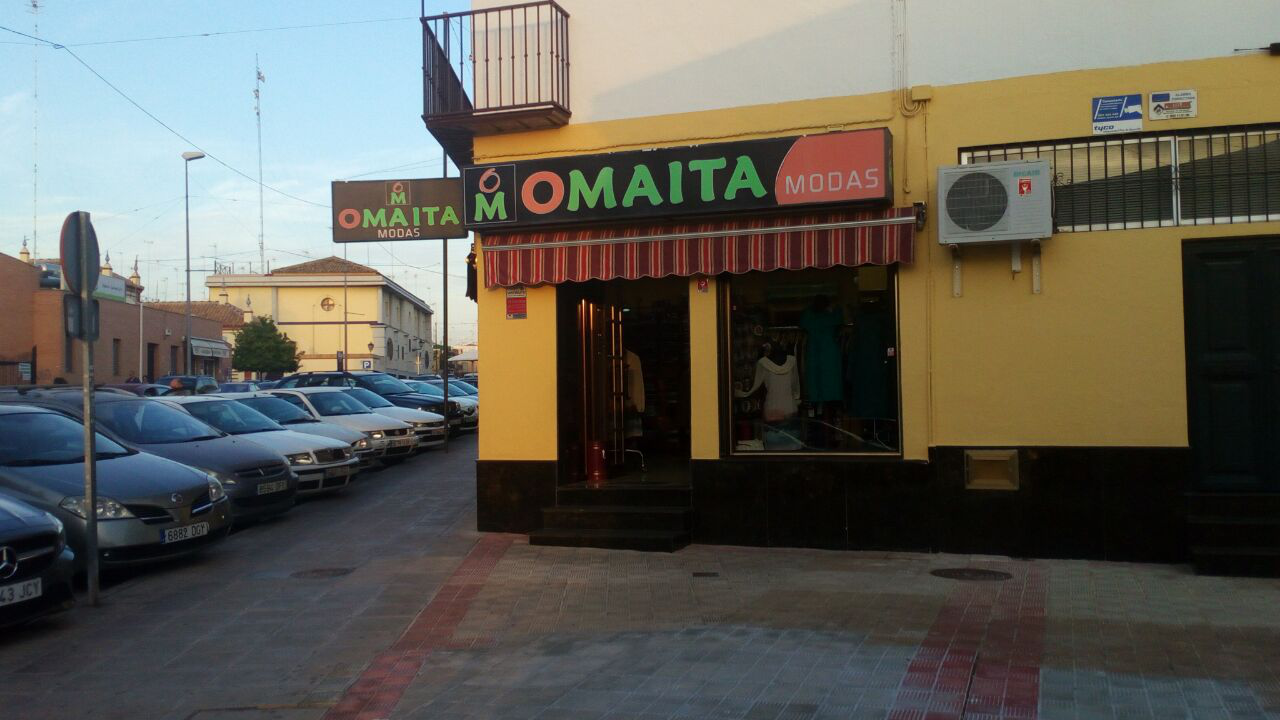
\includegraphics[width=\textwidth, center]{images/tienda1.jpg}

\section{Glosario de Términos}
\begin{table}
	\centering
	\begin{tabularx}{\textwidth}{|l|X|}
		\hline \rowcolor{Gray}
		Término & Descripción \\
		\hline
		Albarán de entrega & Documento obtenido en la recepción del pedido que verifica la correcta entrega del mismo.\\ \hline
		Almacén & Almacén que tienen en común todas las tiendas de la cadena Omaita modas.\\ \hline
		Aviso & Notificación o anuncio dado para comunicar de la falta o limitación. \\ \hline
		Consulta & Actividad que se realiza para tratar de encontrar cualquier entidad almacenada en la base de datos. \\ \hline
		Cadena & Conjunto de tiendas relacionadas entre sí que ofrecen una mezcla estándar de productos, las cuales disponen de almacenes en común. \\ \hline
		Categoría & Tipo de producto que hay en la tienda. \\ \hline
		Emplazamiento & Inmueble de la cadena, puede ser una tienda o el almacén \\ \hline
		Factura & Documento en el que se plasman las compras realizadas además del número de referencia en la base de datos a la lista de compras.\\ \hline
		Pedido & Petición de productos de un emplazamiento al proveedor. \\ \hline
		Proveedor & Entidad económica a la cual varias empresas le compran el material que usarán en la misma o que luego lo venderán al por menor. \\ \hline
		Solicitud & Petición de traspaso de un emplazamiento a otro \\ \hline
		Stock & Conjunto de mercancías o productos que se tienen almacenados en espera de su venta o comercialización. \\ \hline
		Stock mínimo & 5 unidades de un producto almacenadas \\ \hline
		Traspaso & Transferencia de uno o varios productos de un emplazamiento a otro \\ \hline
	\end{tabularx}
\end{table}

\begin{landscape}
\section{Modelo de negocio}

\subsection{Proceso de venta}
\begin{figure}[H]
	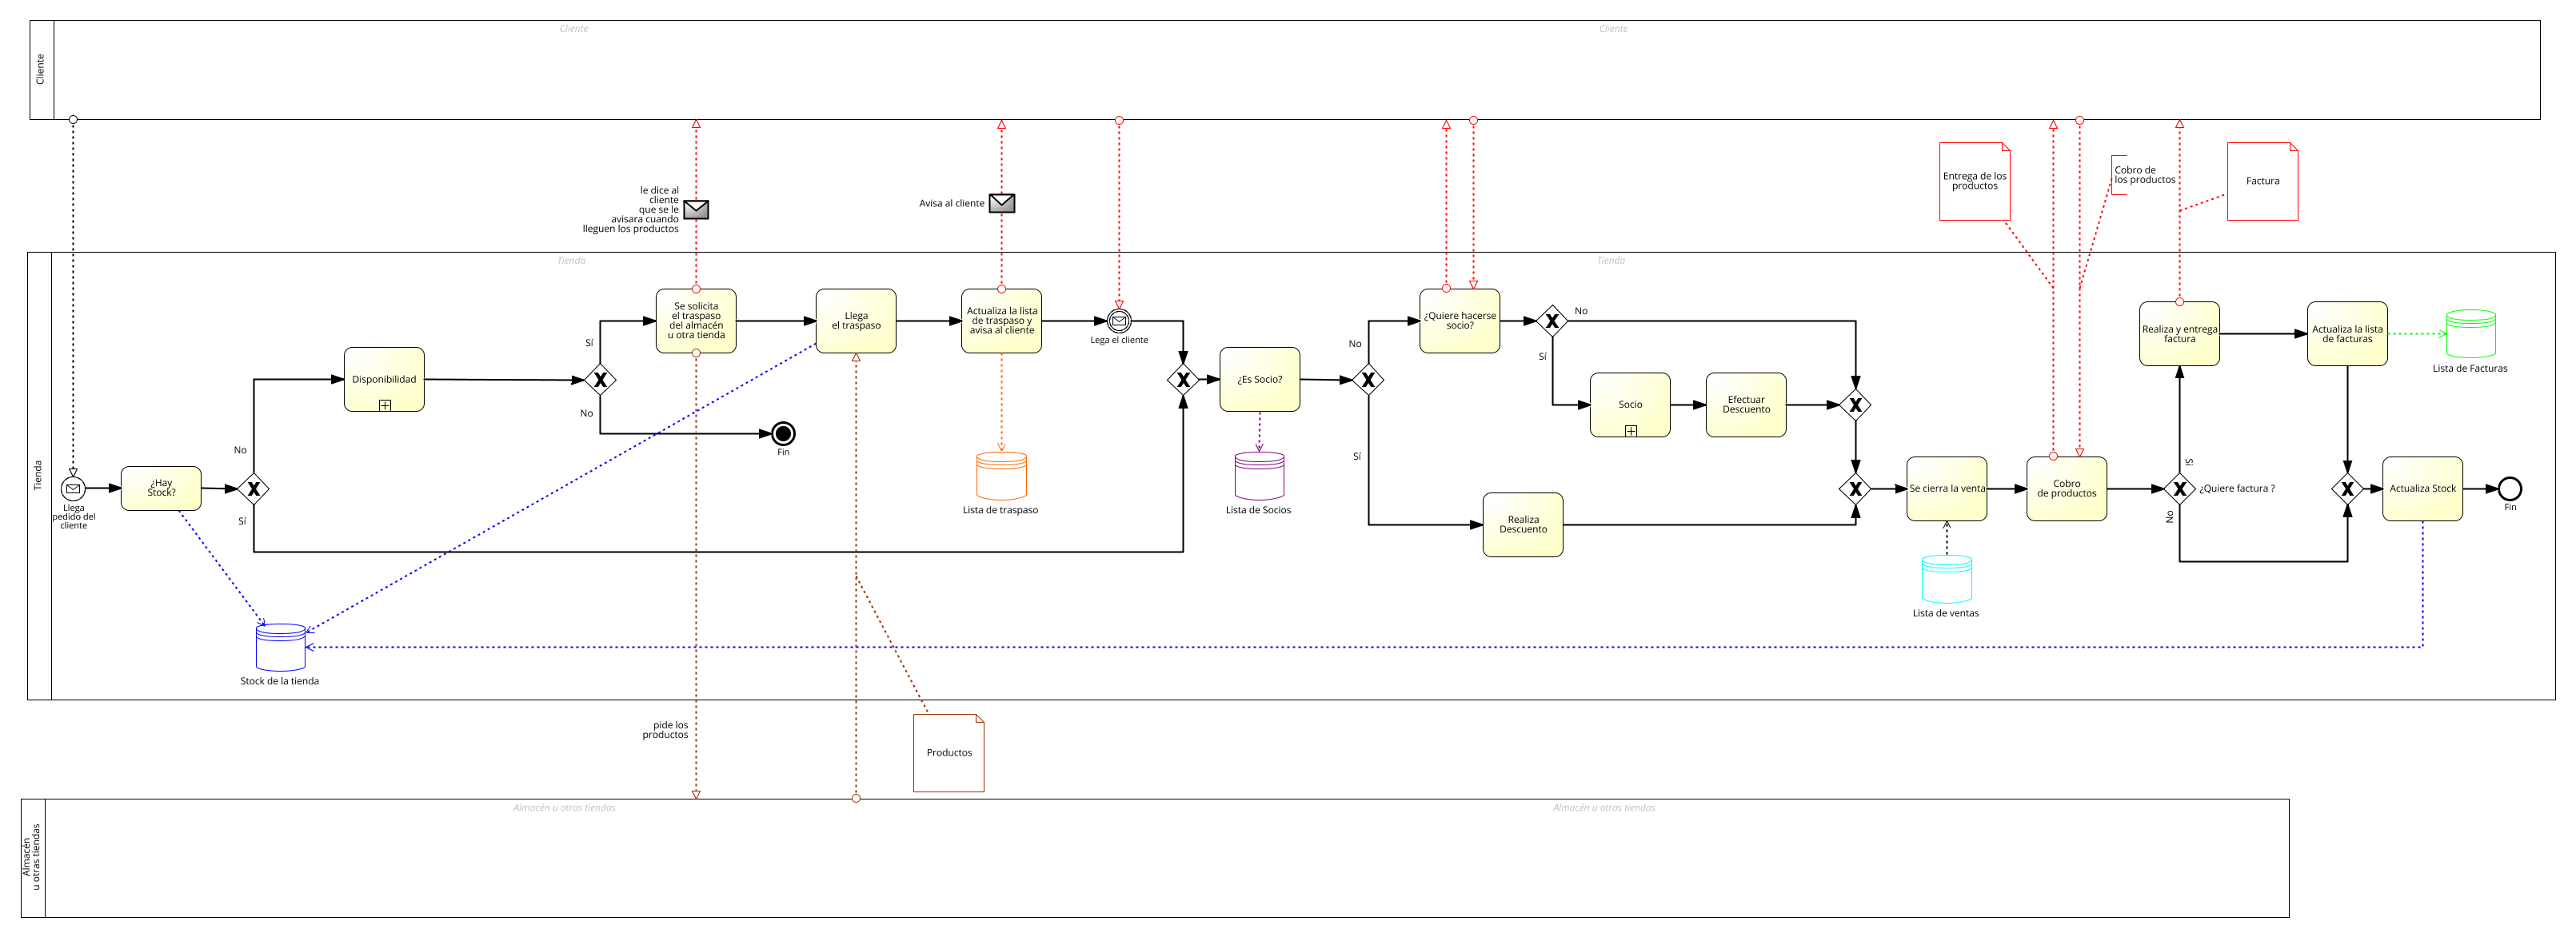
\includegraphics[width=\paperwidth, center]{images/bpmn/proceso-venta.png}
	\caption{Proceso de venta}
\end{figure}
%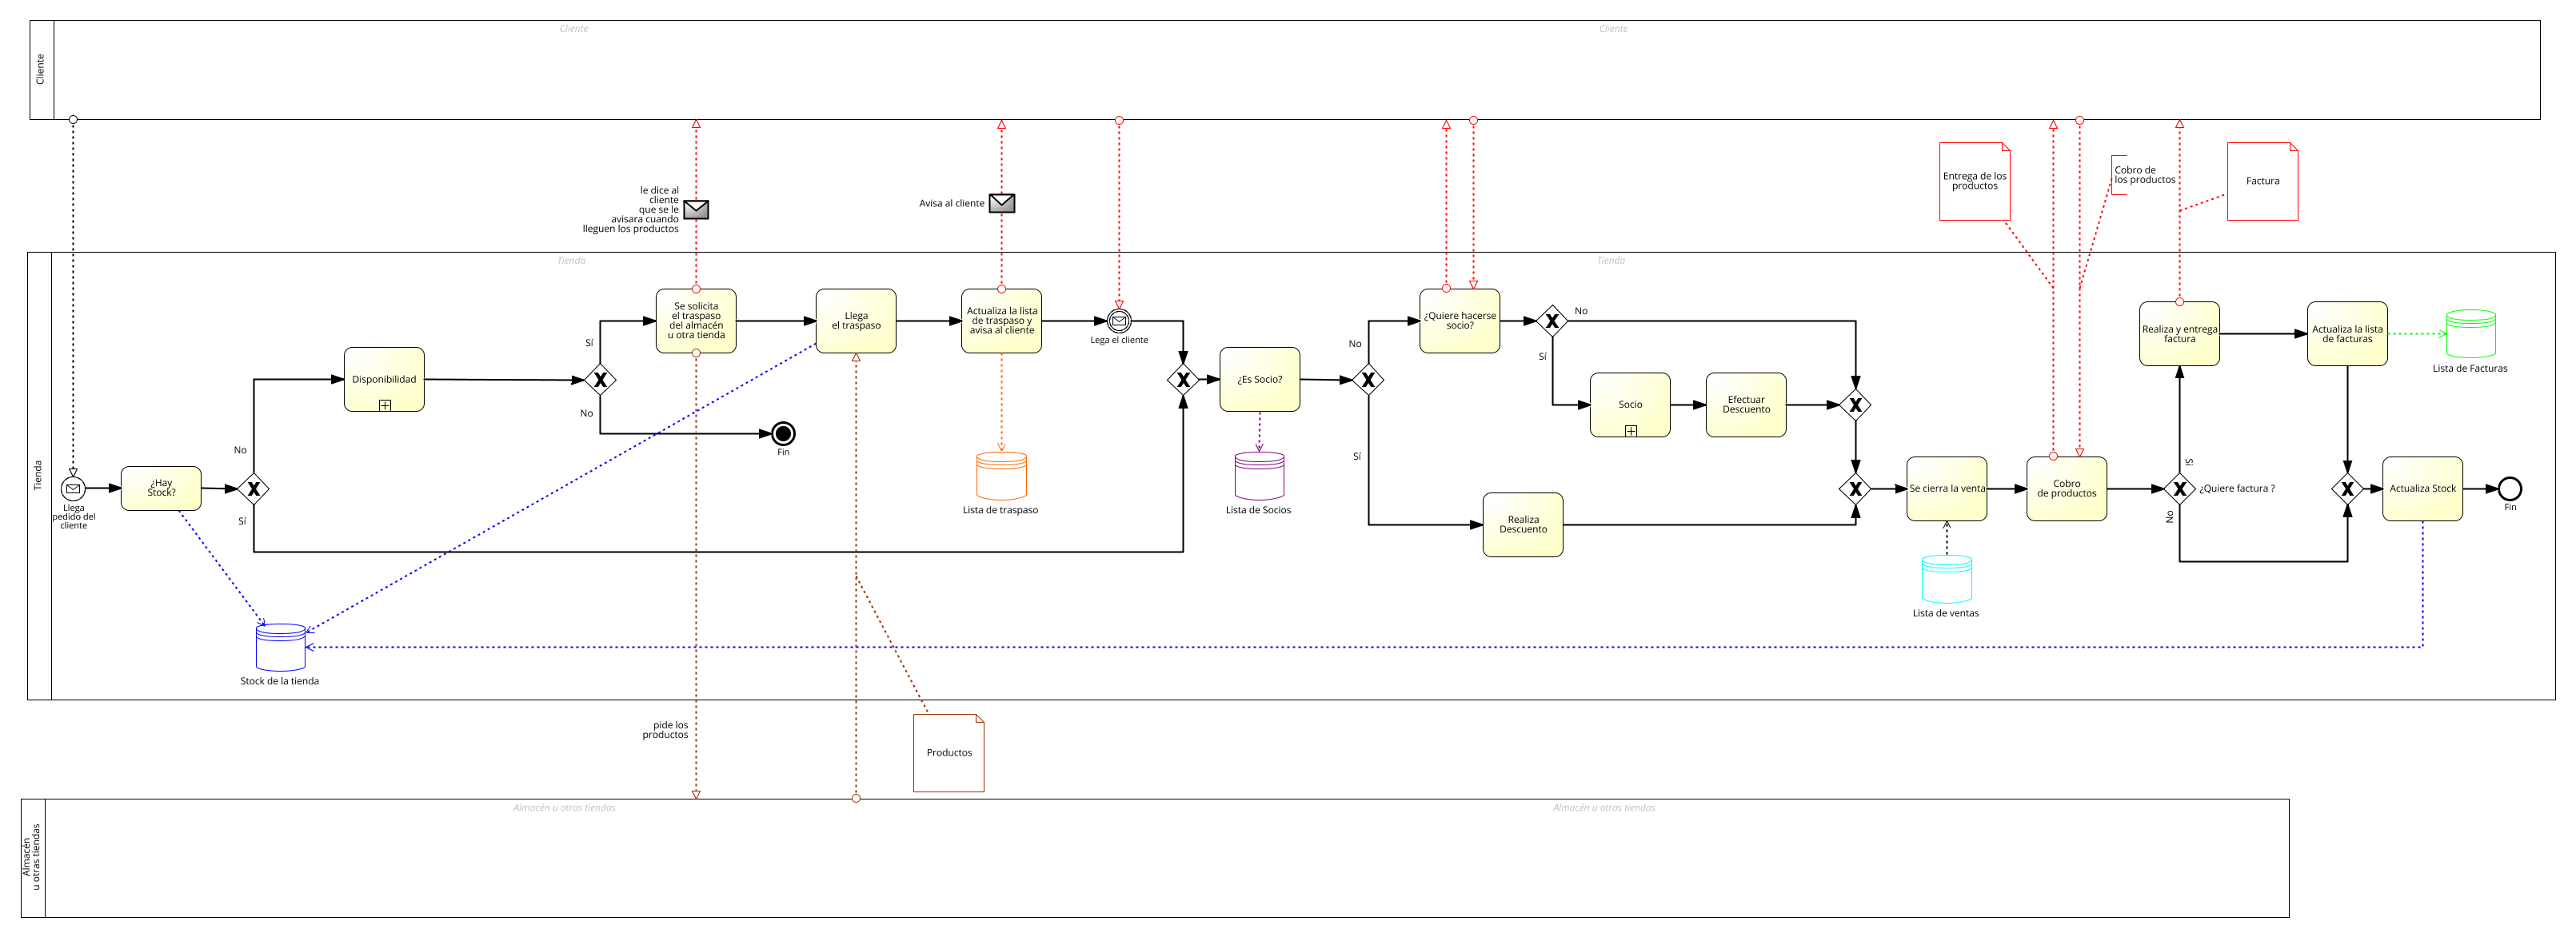
\includegraphics[width=\paperwidth, center]{images/bpmn/proceso-venta.png}
\subsection{Proceso de compra al proveedor}
\pagenumbering{gobble}
\begin{figure}[H]
	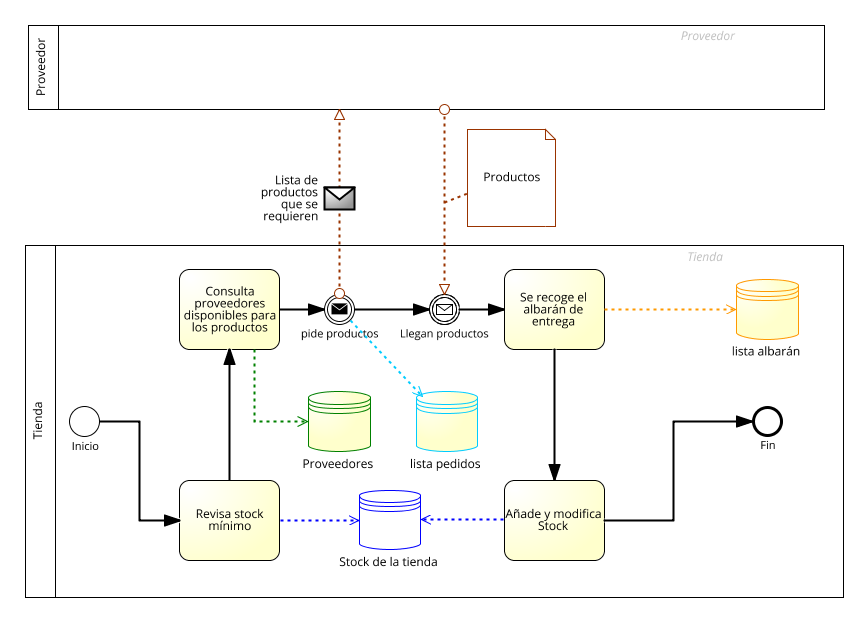
\includegraphics[width=\paperwidth, center]{images/bpmn/proceso-proveedor.png}
	\caption{Proceso de compra al proveedor}
\end{figure}
%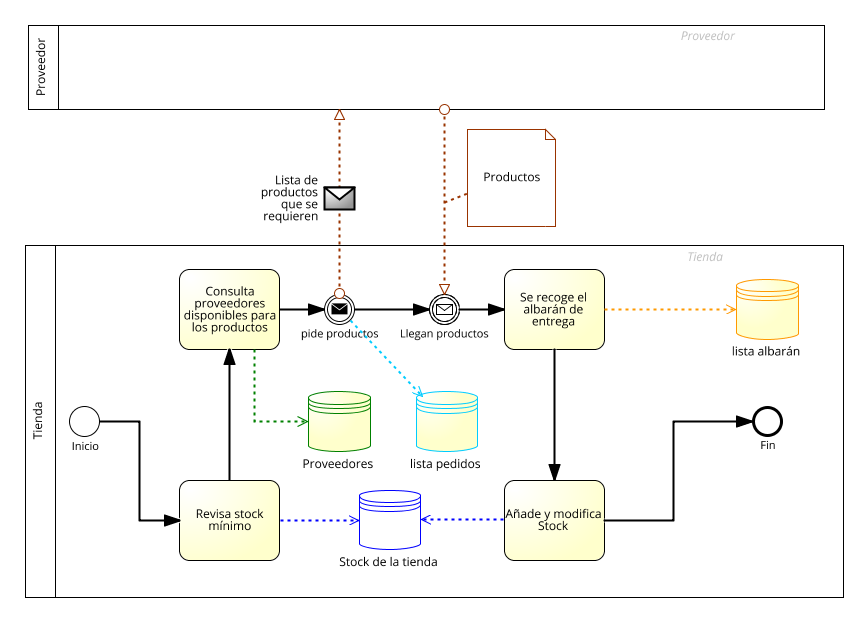
\includegraphics[width=\paperwidth, center]{images/bpmn/proceso-proveedor.png}

\subsection{Proceso de disponibilidad}
\begin{figure}[H]
	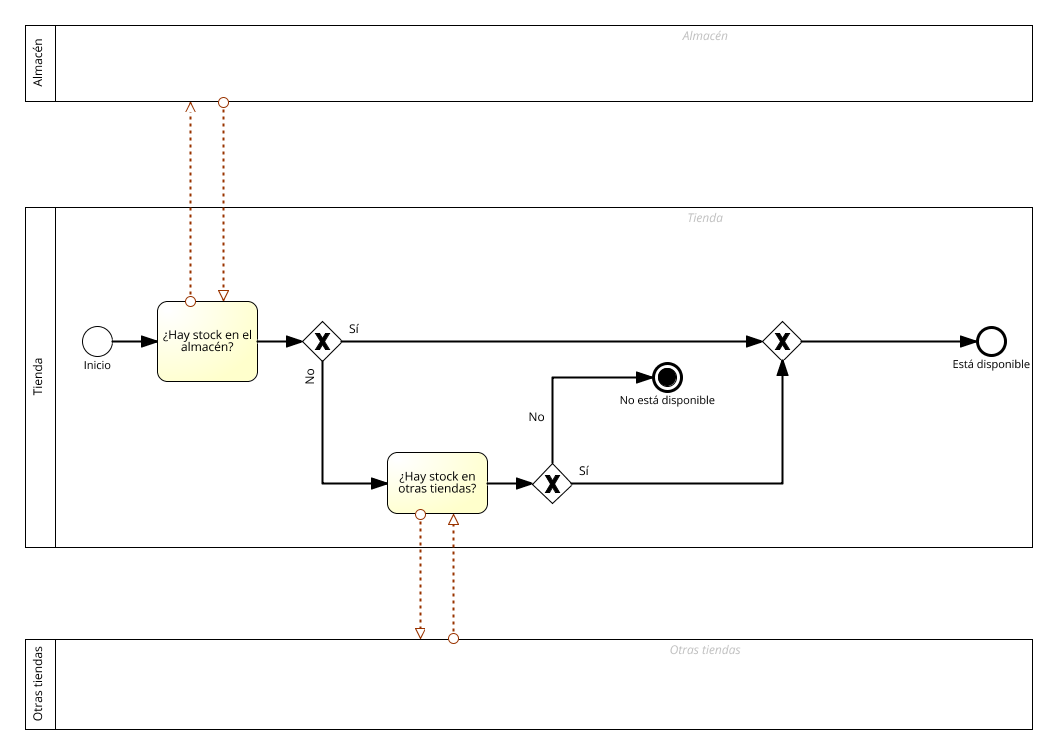
\includegraphics[width=\paperwidth, center]{images/bpmn/disponibilidad .png}
	\caption{Proceso de disponibilidad}
\end{figure}
%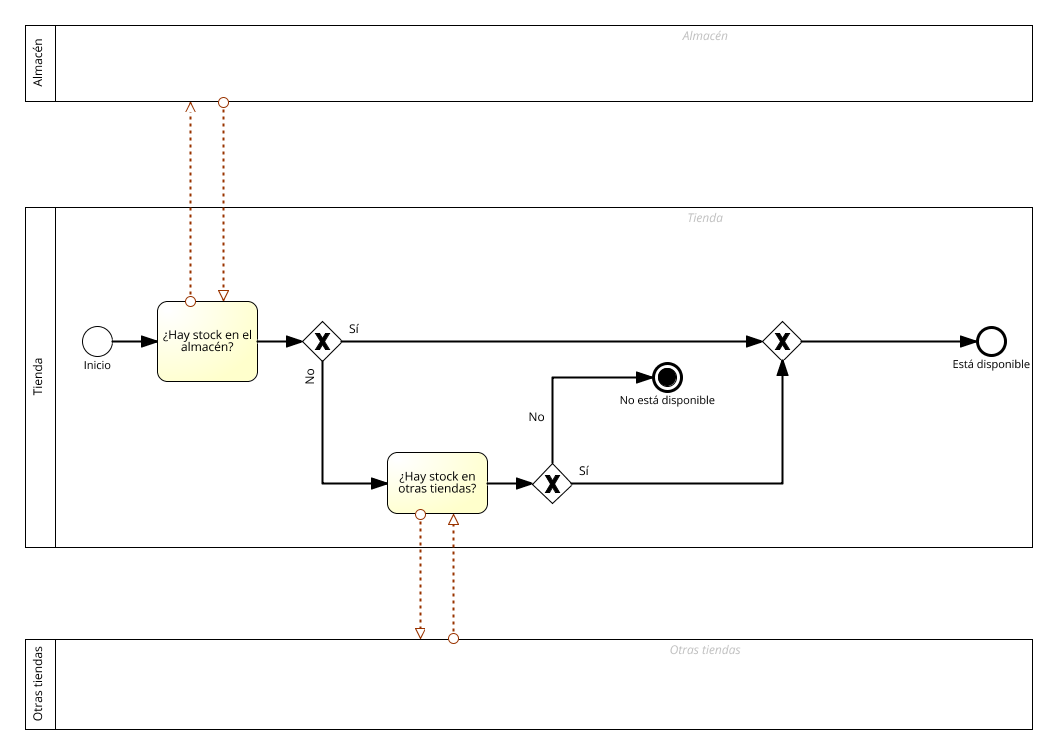
\includegraphics[width=\paperwidth, center]{images/bpmn/disponibilidad .png}

\subsection{Proceso de creación de socios}
\begin{figure}[H]
	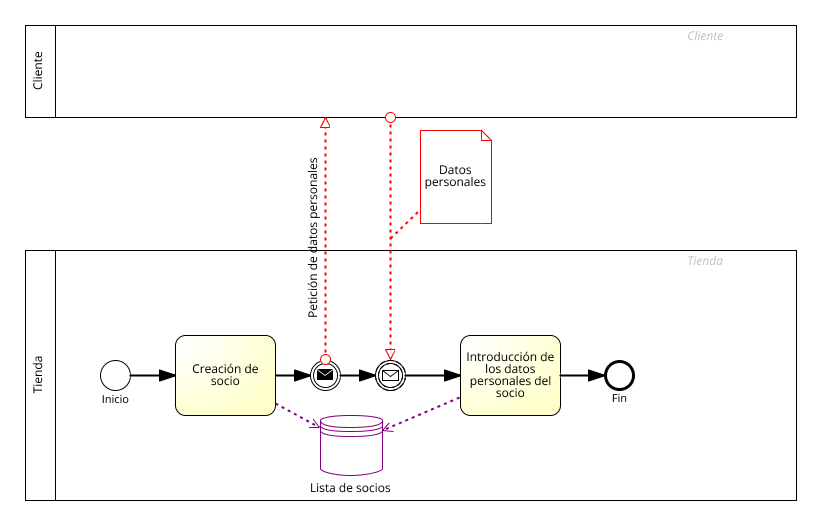
\includegraphics[width=\paperwidth, center]{images/bpmn/socios .png}
	\caption{Proceso de creación de socios}
\end{figure}
%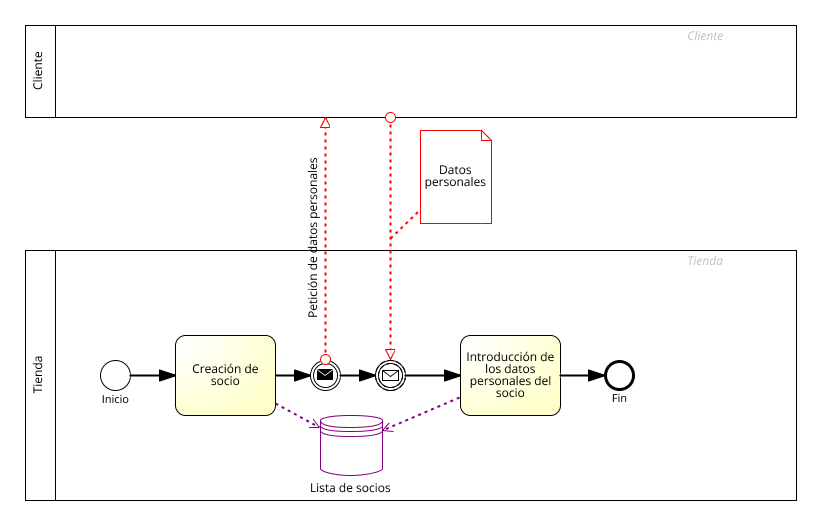
\includegraphics[width=\paperwidth, center]{images/bpmn/socios .png}
\end{landscape}

\section{Visión General del Sistema}
\subsection{Descripción}
Para solucionar los problemas planteados de clientela y gestión, el sistema estará diseñado para permitir la gestión de las ventas, los productos, los pedidos, los traspasos y los clientes de manera más eficaz.
\\\\
El objetivo principal de nuestro cliente es aumentar su clientela con la ayuda de una página web, esto lo haremos desarrollando un catálogo online de la tienda para que los clientes puedan consultar o comprar cualquier producto en cualquier momento, además de facilitar la gestión interna de la cadena.
\\\\
Con todo esto principalmente lo que se quiere es aumentar los beneficios y hacer más eficiente la gestión de la cadena.

\section{Catálogo de requisitos}

\begin{figure}[H]
	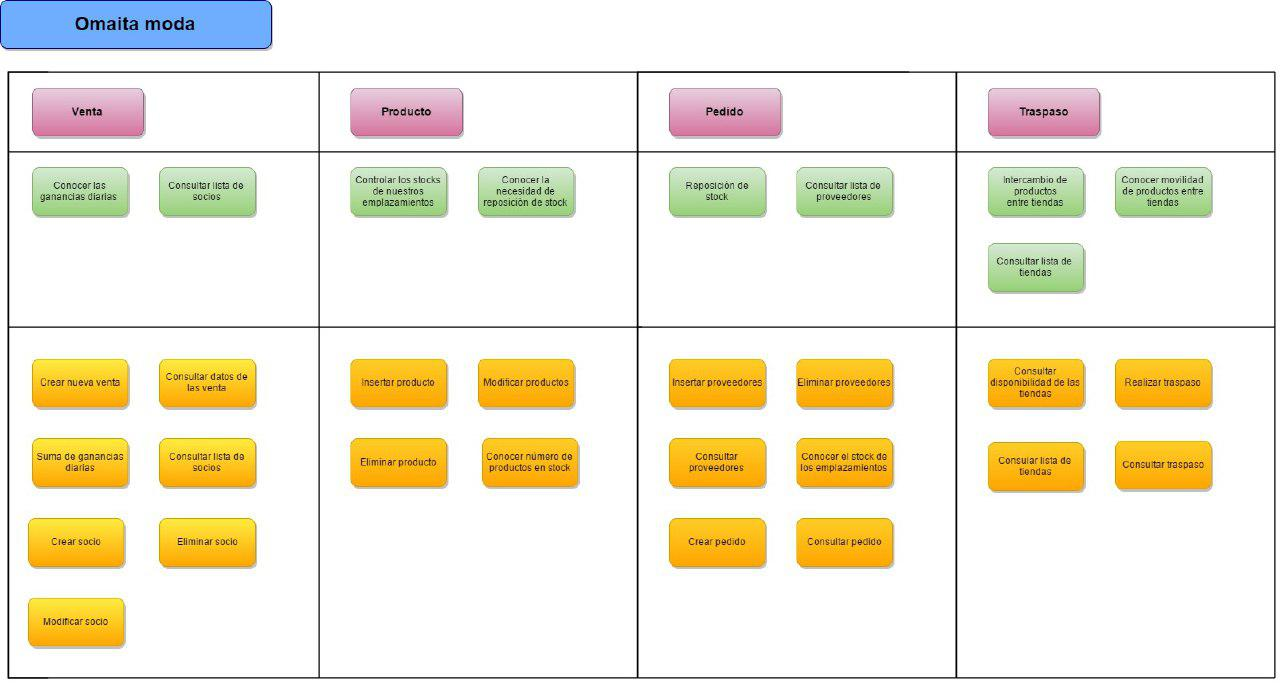
\includegraphics[width=\linewidth]{images/MapaRequisitos.jpg}
	\caption{Mapa de requisitos}
\end{figure}

\subsection{Requisitos generales}

\requit{RG-01}{Gestion ventas}{Propietario de la cadena}{poder gestionar y consultar las ventas de las tiendas}{llevar una buena gestión de ellas}
\requit{RG-02}{Gestion proveedores}{Propietario de la cadena}{poder gestionar y consultar los pedidos a proveedores}{llevar una buena gestión de ellos}
\requit{RG-03}{Traspasos}{Propietario de la cadena}{que haya un sistema de traspasos}{poder aprovechar al máximo el stock de las tiendas}
\requit{RG-04}{Catálogo}{Cliente}{poder ver una lista de los productos ofrecidos y disponibles}{realizar mis compras}

\subsection{Requisitos de información}

\requit{RI-01}{Información sobre ventas}{Propietario de la cadena}{que el sistema almacene la información correspondiente a las ventas, guardando así los siguientes datos
	\begin{itemize}
		\item Precio total de la venta.
		\item Fecha en la que se llevó acabo la venta.
		\item La relación entre producto y venta que almacenará: el producto vendido, el precio y el IVA del mismo en el momento en el que se vendió.
	\end{itemize}}{conocer los datos de las ventas realizadas.}

\requit{RI-02}{Información sobre facturas}{propietario de la cadena}{que el sistema almacene la información correspondiente a las facturas, guardando así los siguientes datos:
	
	\begin{itemize}
		\item Precio final de la venta.
		\item Fecha en la que se tramita la factura.
		\item Número de la factura.
		\item Un campo llamado devuelto, usado para las devoluciones, si el campo tiene el valor false, entonces podemos contabilizar esa factura sin problemas, si el campo tiene el valor true significará que el dinero fue devuelto al cliente y por la tanto no podríamos contabilizarlo.
\end{itemize}}{conocer los datos de las facturas expedidas.}

\requit{RI-03}{Información sobre socios}{propietario de la cadena}{que el sistema almacene la información de los clientes que son socios, guardando los siguientes datos en él:
	\begin{itemize}
		\item Nombre.
	 	\item Apellidos.
		\item DNI.
		\item Dirección.
		\item Fecha de Nacimiento.
		\item Email.
\end{itemize}}{llevar un control de los clientes que son socios y así poderles aplicar descuentos en sus compras.}

\requit{RI-04}{Información sobre productos}{propietario de la cadena}{que los productos que venda la cadena se guarden con las siguientes características en el sistema:
	\begin{itemize}
		\item Nombre.
		\item Una breve descripción.
		\item La categoría del producto: abrigos, chaquetas, camisas, camisetas, jersey, vestidos, faldas, pantalones, calzado, accesorios y bisutería.
		\item Precio del producto.
		\item IVA actual, para controlar el IVA en todo momento
	\end{itemize}}{conocer los datos de cada producto.}

\requit{RI-05}{Stock del producto}{propietario de la cadena}{saber el stock de cada producto en cada tienda de la cadena y del almacén}{controlar el stock de la cadena}

\requit{RI-06}{Información sobre los emplazamientos}{propietario de la cadena}{guardar la dirección de las tiendas y del almacén de la cadena, además de su teléfono de contacto}{conocer la localización de las mismas}

\requit{RI-07}{Información sobre los proveedores}{propietario de la cadena}{disponer de la siguiente información sobre proveedores:
	\begin{itemize}
		\item Nombre.
		\item CIF.
		\item Número de teléfono.
		\item Email.
	\end{itemize}}{saber a qué proveedores puede realizar los pedidos}

\requit{RI-08}{Información sobre los pedidos}{propietario de la cadena}{que el sistema almacene los pedidos guardando los siguientes datos:
	\begin{itemize}
		\item Fecha en la que se realiza.
		\item Precio total del pedido.
		\item Una asociación que controla la cantidad de cada producto del pedido, el precio y el IVA.
	\end{itemize}}{conocer los datos de los pedidos realizados.}

\requit{RI-09}{Información sobre traspasos}{propietario de la cadena}{que el sistema guarde los traspasos almacenando los siguientes datos:
	\begin{itemize}
		\item Fecha de traspaso.
		\item Asociación que controla la cantidad de cada producto en el traspaso.
	\end{itemize}}{conocer los datos de los traspasos realizados.}

\requit{RI-10}{Información sobre el albarán}{propietario de la cadena}{que el sistema almacene información correspondiente a los albaranes, guardando así los siguientes datos
	\begin{itemize}
		\item Fecha de firma del albarán.
		\item Precio total.
	\end{itemize}}{tener un control de los pedidos recibidos los cuales son controlados por los albaranes.}

\requit{RI-11}{Información sobre solicitud}{propietario de la cadena}{que el sistema almacene información correspondiente a las solicitudes de traspaso, guardando así los siguientes datos
	\begin{itemize}
		\item Fecha de solicitud.
		\item Asociación que controla la cantidad de cada producto en la solicitud
\end{itemize}}{conocer los datos de las solicitudes realizadas.}

\subsection{Requisitos funcionales}

\requit{RF-01}{Crear ventas}{empleado}{poder crear y consultar ventas realizadas}{poder así conocer las ganancias de la tienda}

\requit{RF-02}{Actualizar stocks tras venta}{propietario de la cadena}{que tras una factura asociada a una venta el stock se actualice}{controlar el stock de manera correcta}

\requit{RF-03}{Crear socios}{empleado}{poder crear socios en una lista y poder consultarla}{llevar así un control sobre estos y saber si se tiene que aplicar o no el descuento.}

\requit{RF-04}{Modificar socios}{empleado}{poder modificar la dirección y el email de un socio ya creado}{tener los datos correctos del socio.}

\requit{RF-05}{Eliminar socios}{empleado}{poder eliminar un socio de la base de datos}{dejar de tener almacenados los datos de un cliente que desiste de su derecho de ser socio.}

\requit{RF-06}{Crear, modificar y eliminar productos}{empleado}{poder insertar, modificar la descripción, el precio y el IVA de un producto, o eliminar un producto de mi base de datos}{poder así llevar una buena gestión de los productos.}

\requit{RF-07}{Crear y modificar stocks}{empleado}{poder crear el stock de un producto y modificar su cantidad}{llevar un control sobre la disponibilidad de los productos según su emplazamiento.}

\requit{RF-08}{Crear, modificar y eliminar proveedores}{propietario de la cadena}{poder insertar, modificar el nombre, el email y el teléfono, o eliminar proveedores en mi base de datos}{conocer los proveedores disponibles y tener sus datos actualizados.}

\requit{RF-09}{Crear pedidos}{empleado}{poder crear pedidos}{tener constancia de todos los pedidos realizados por cada uno de mis emplazamientos}

\requit{RF-10}{Actualizar stock tras pedido}{propietario de la cadena}{que tras recibir el albarán que confirma la entrega del pedido el stock se actualice}{controlar correctamente el stock.}

\requit{RF-11}{Crear solicitud de traspaso}{empleado}{poder crear una solicitud de traspaso}{así poder pedir a otra tienda productos que necesite.}

\requit{RF-12}{Crear traspasos}{empleado}{poder crear traspasos}{responder a la necesidad de las solicitudes de traspaso.}

\requit{RF-13}{Actualizar stock tras traspaso}{propietario de la cadena}{que cuando se realice un traspaso, se modifiquen de manera correcta los stocks de las tiendas implicadas}{así poder tener una buena gestión sobre nuestros stocks}

\requit{RF-14}{Consultar traspasos}{propietario de la cadena}{poder consultar todos los traspasos realizados por mis emplazamientos}{conocer la movilidad de los productos entre estos.}

\requit{RF-15}{Crear y eliminar emplazamientos}{propietario de la cadena}{poder añadir o eliminar emplazamientos en la base de datos}{saber que emplazamientos están en la cadena.}

\requit{RF-16}{Modificar emplazamientos}{propietario de la cadena}{poder modificar la dirección y el número de teléfono de un emplazamiento}{tener los datos actualizados de mis emplazamientos.}

\requit{RF-17}{Devolución}{propietario de la cadena}{que cuando se realiza una devolución el campo devuelto de las facturas pase a ser True, y si es necesario que el empleado cree de nuevo toda la venta y la factura pero sin los productos devueltos, esta factura deberá tener el campo devuelto como False}{tener un control sobre las devoluciones.}

\requit{RF-18}{Crear albarán}{empleado}{crear una copia del albarán de entrega que me ha dado el proveedor al traer el pedido que habíamos hecho}{tener la información de los albaranes recogida en la base de datos.}


\subsection{Requisitos no funcionales}

\requit{RNF-01}{Acceso al sistema}{propietario de la cadena}{que todos mis empleados tengan acceso al sistema}{facilitar la gestión de las tiendas y el control del sistema.}

\requit{RNF-02}{Protección de datos socios}{propietario de la cadena}{que los datos de los socios permanezcan privados y seguros}{cumplir la Ley de Protección de Datos}

\requit{RNF-03}{Mantenimiento}{propietario de la cadena}{realizar el mantenimiento del sistema al menos una vez al mes}{prevenir problemas mayores en el sistema.}

\subsection{Reglas de negocio}

\requit{RN-01}{Descuento a socios}{propietario de la cadena}{aplicar un 5\% de descuento en las ventas realizadas a socios}{recompensar su fidelidad}

\requit{RN-02}{Tamaño mínimo de pedidos}{propietario de la cadena quiero}{que los pedidos sean como mínimo de 20 unidades por producto}{abaratar gastos de transporte.}

\requit{RN-03}{Evitar traspaso si se provoca stock mínimo}{propietario de la cadena}{que las tiendas no puedan ofrecer el traspaso de un producto, si debido al traspaso el producto llega a su stock mínimo}{evitar que éstas se queden desabastecidas}

\requit{RN-04}{Política de devoluciones}{propietario de la cadena}{que solo se acepten devoluciones, con un plazo máximo de 30 días después de la compra}{dificultar la devolución de productos usados}

\requit{RN-05}{Aviso stock mínimo}{trabajador de una tienda}{obtener un aviso cuando el stock de un producto llegue al stock mínimo}{evitar el desabastecimiento de un producto}

\section{Pruebas de aceptación}

\textbf{PA-01 Ventas}:
\begin{itemize}
	\item Se realiza una venta y con una consulta vemos que la fecha y el precio total es el esperado.
\end{itemize}

\textbf{PA-02 Facturas y Devoluciones}:
\begin{itemize}
	\item Se realiza una factura y con una consulta vemos que el precio final de la venta, la fecha, el número de la factura y el IVA es el esperado.
	\item Un cliente devuelve un producto dentro del plazo de 30 días y por tanto se devuelve el dinero al cliente, realizamos una consulta sobre la factura del producto devuelto y vemos la factura original con el campo devuelto como True.
	\item Tras la situación anterior el trabajador crea una nueva factura con todos los productos originales de la compra menos con el que se ha devuelto, entonces se realiza una consulta a la factura y vemos como se ha eliminado correctamente el producto devuelto y no se ha contabilizado en el precio de la factura. (Situación que solo se da si el producto devuelto pertenece a una factura de más productos)
	\item Un cliente desea devolver un producto tras 30 días de su compra, los artículos no pueden ser devueltos debido a que ha pasado más de 30 días desde su compra.
\end{itemize}

\textbf{PA-03 Socios}:
\begin{itemize}
	\item Se añade un nuevo socio, se actualiza la lista de socios y este aparece con todos los siguientes datos: nombre, apellidos, DNI, dirección, fecha de nacimiento y email.
	\item Se elimina un socio, se actualiza la lista de socios y en ella no aparece el socio.
	\item Se modifica los datos de un socio, se actualiza la lista de socios y este aparece con sus datos modificados.
	\item Se intenta añadir un nuevo socio, pero le faltan datos, el sistema no permite añadirlo.
	\item Se intentar añadir un nuevo socio, pero ya está en la base de datos y el sistema no nos lo permite.
\end{itemize}

\textbf{PA-04 Productos}:
\begin{itemize}
	\item Se añade un nuevo producto, se actualiza la lista de productos y este aparece con todos los siguientes datos: nombre, descripción, categoría, precio del producto e IVA.
	\item Se elimina un producto, se actualiza la lista de productos y en ella no aparece el producto eliminado.
	\item Se modifica los datos de un producto, se actualiza la lista de productos y este aparece con sus datos modificados.
	\item Se intenta añadir un producto nuevo, pero le faltan datos, el sistema no permite añadirlo.
	\item Se desea añadir un producto que ya está en la base de datos y el sistema no nos lo permite.
\end{itemize}

\textbf{PA-05 Stock}:
\begin{itemize}
	\item Si el stock de un producto es de 10 y un cliente quiere comprar 11, el stock es superado y el sistema no permite esa compra.
	\item Si el stock de un producto es de 10 y un cliente quiere comprar 3, se le permite la venta y se modifica el stock en la base de datos.
	\item Se realiza un traspaso entre 2 emplazamientos, hacemos 2 consultas y comprobamos que el stock de cada emplazamiento es el correcto tras la transacción.
	\item El stock de un producto es de 6 y un cliente realiza una compra de ese producto, entonces se muestra un aviso de que el stock de ese producto ha alcanzado el stock mínimo.
	\item Consultamos el stock de la tienda y después recibimos el albarán del pedido que habíamos realizado, consultamos de nuevo el stock y vemos que se ha actualizado correctamente.
\end{itemize}

\textbf{PA-06 Proveedores}:
\begin{itemize}
	\item Se registra un proveedor nuevo, se actualiza la lista de proveedores y aparece el proveedor con los siguientes datos: nombre, CIF, número de teléfono y email.
	\item Se modifican los datos de un proveedor, se actualiza la lista de proveedores y sale el proveedor con los datos modificados.
	\item Se elimina un proveedor, al actualizar la lista de los proveedores, el proveedor eliminado ya no aparece.
	\item Se intenta añadir un proveedor que ya está en la base de datos y el sistema no lo permite.
\end{itemize}

\textbf{PA-07 Pedidos y albaranes}:
\begin{itemize}
	\item El almacén ha llegado a stock mínimo de algunos de sus productos y se realiza un pedido al proveedor o proveedores, tras recibir los productos del proveedor hacemos una consulta para ver el albarán está en orden y que los productos del pedido son los que se solicitaron.
	\item Se realiza una consulta sobre el pedido que se había realizado y vemos que se muestran los siguientes datos: fecha en la que se realizó, precio total y emplazamiento que realizó el pedido.
	\item Se intenta realizar un pedido de 15 unidades y salta un mensaje de error, ya que el pedido tiene que ser de 20 unidades mínimo.
	\item Se crea un albarán con los datos recibidos del albarán de entrega y hacemos una consulta para ver que se muestra correctamente.
\end{itemize}

\textbf{PA-08 Traspasos y solicitudes}:
\begin{itemize}
	\item Falta stock de un producto y se solicita a otro emplazamiento, el otro emplazamiento realiza el traspaso y se reciben los productos. Hacemos una consulta para la solicitud y otra consulta para traspaso y vemos que los productos son correctos, además de que aparecen las respectivas fechas y los emplazamientos de la relación.
	\item Se intenta solicitar un traspaso de 3 unidades de un producto a una tienda, pero la tienda a la que se solicita el traspaso solo posee 6 unidades del producto por lo que salta un mensaje de que no se puede solicitar el traspaso a esta tienda.
\end{itemize}

\textbf{PA-09 Emplazamientos}:
\begin{itemize}
	\item Se añade una nueva tienda, se realiza una consulta y vemos que se ha añadido correctamente.
	\item Se cambia la localización del almacén, se realiza una consulta y vemos que se ha cambiado correctamente.
	\item Se elimina una tienda, se realiza una consulta y vemos que se ha eliminado correctamente y ya no aparece en la lista de emplazamientos.
	\item Se realiza una consulta sobre el stock de una tienda y este se muestra correctamente.
\end{itemize}

\textbf{PA-10 Descuentos}:
\begin{itemize}
	\item Un socio va a gastar un total de 100 euros en nuestros productos, al ser socio se le aplica un descuento del 5\%, por tanto, se le rebajan 5 euros en la factura.
	\item Un cliente va a gastar un total de 50 euros, al no ser socio no se le aplica el descuento y tiene que pagar los 50 euros completos.
\end{itemize}

\textbf{PA-11 Tamaño mínimo pedidos}:
\begin{itemize}
	\item Se desea realizar un pedido de 10 productos y de cada producto se requieren 20 unidades, por tanto, se puede hacer el pedido.
	\item Se desea realizar el pedido de un producto con una cantidad equivalente a 15, este pedido no se podría llevar a cabo debido a que no llega a las 20 unidades necesarias.
\end{itemize}


\section{Modelo Conceptual}
\subsection{Diagramas de clases UML}

\begin{figure}[H]
	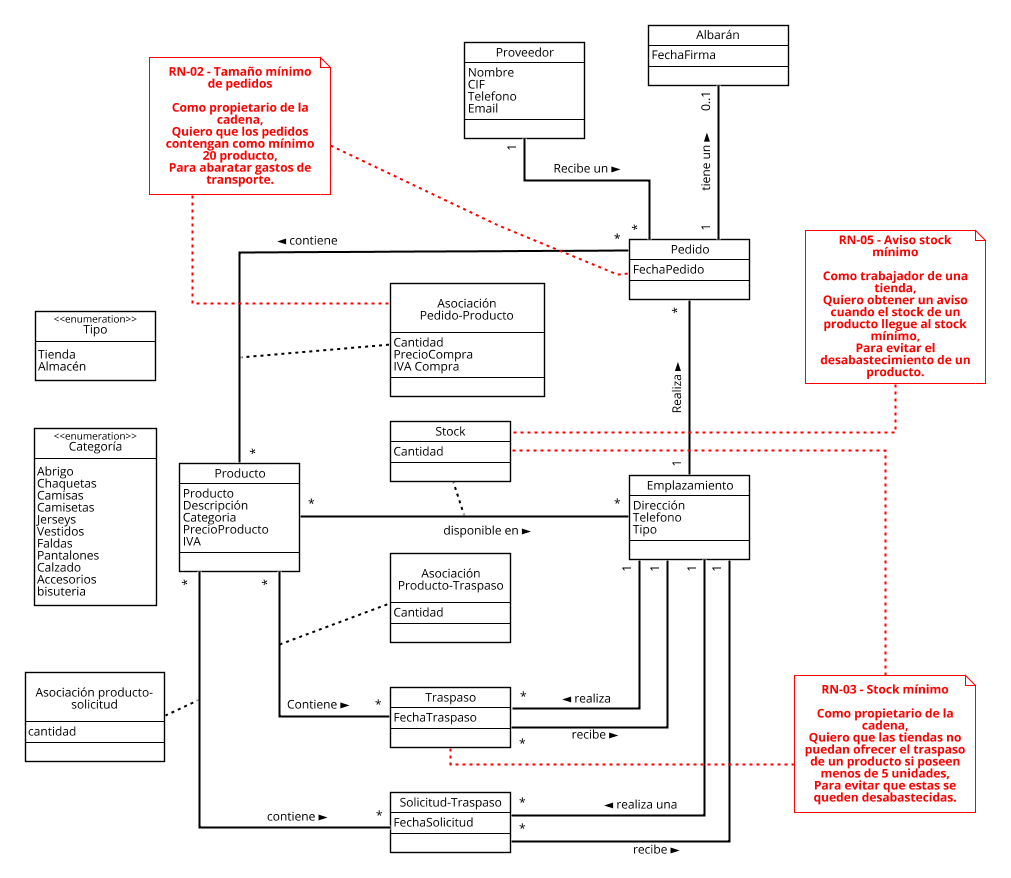
\includegraphics[width=\linewidth]{images/UML-traspaso-pedido.png}
	\caption{UML Traspaso / Pedido}
\end{figure}

\begin{figure}[H]
	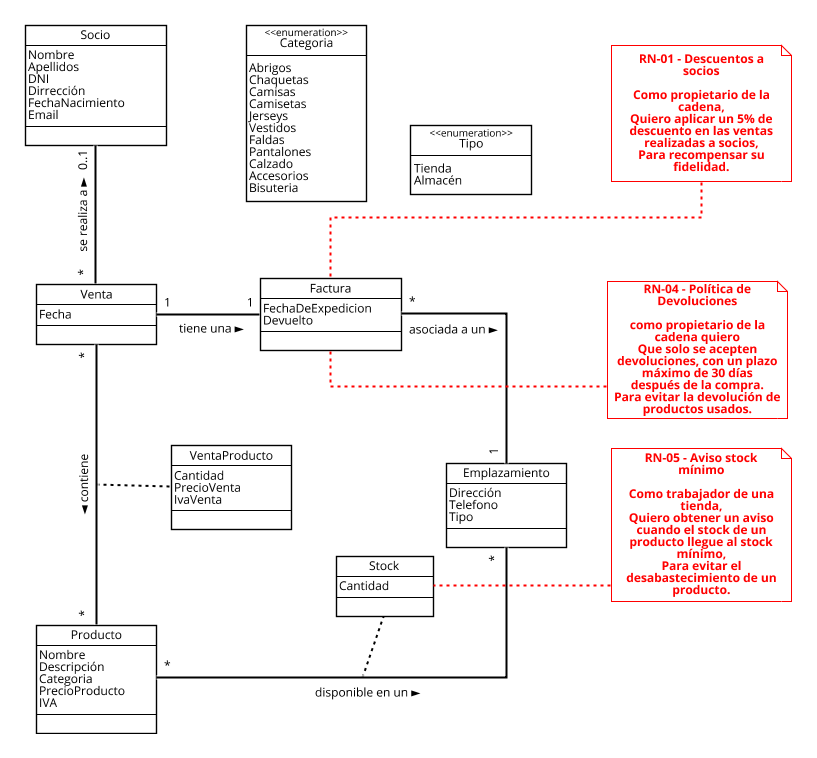
\includegraphics[width=\linewidth]{images/UML-venta.png}
	\caption{UML Venta}
\end{figure}

\subsection{Escenarios de prueba}

\begin{figure}[H]
	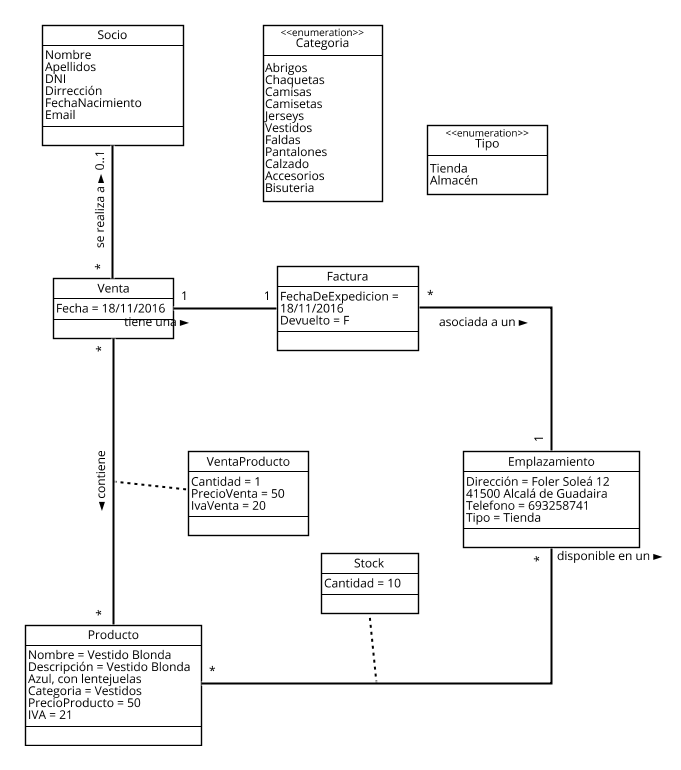
\includegraphics[width=\linewidth]{images/pruebas/venta-no-socio.png}
	\caption{UML Venta NO Socio}
\end{figure}

\begin{figure}[H]
	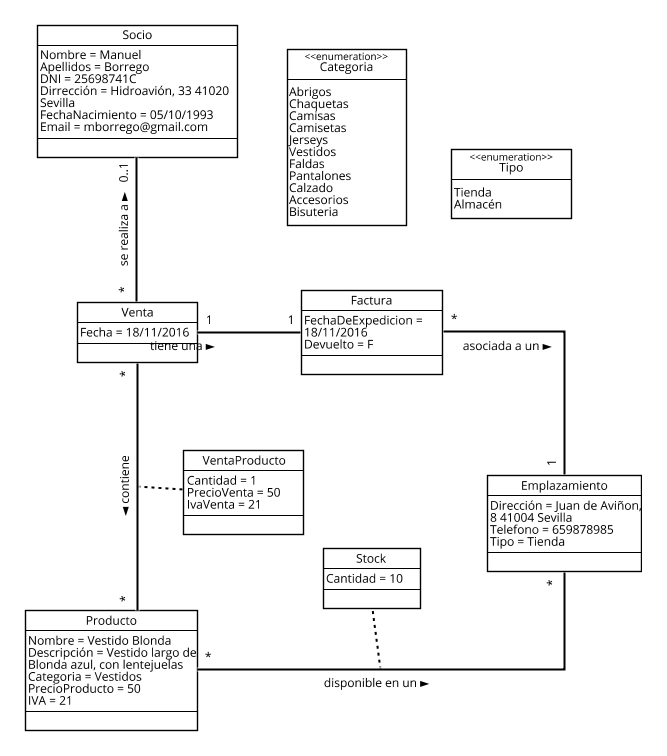
\includegraphics[width=\linewidth]{images/pruebas/venta-socio.png}
	\caption{UML Venta Socio}
\end{figure}

\begin{figure}[H]
	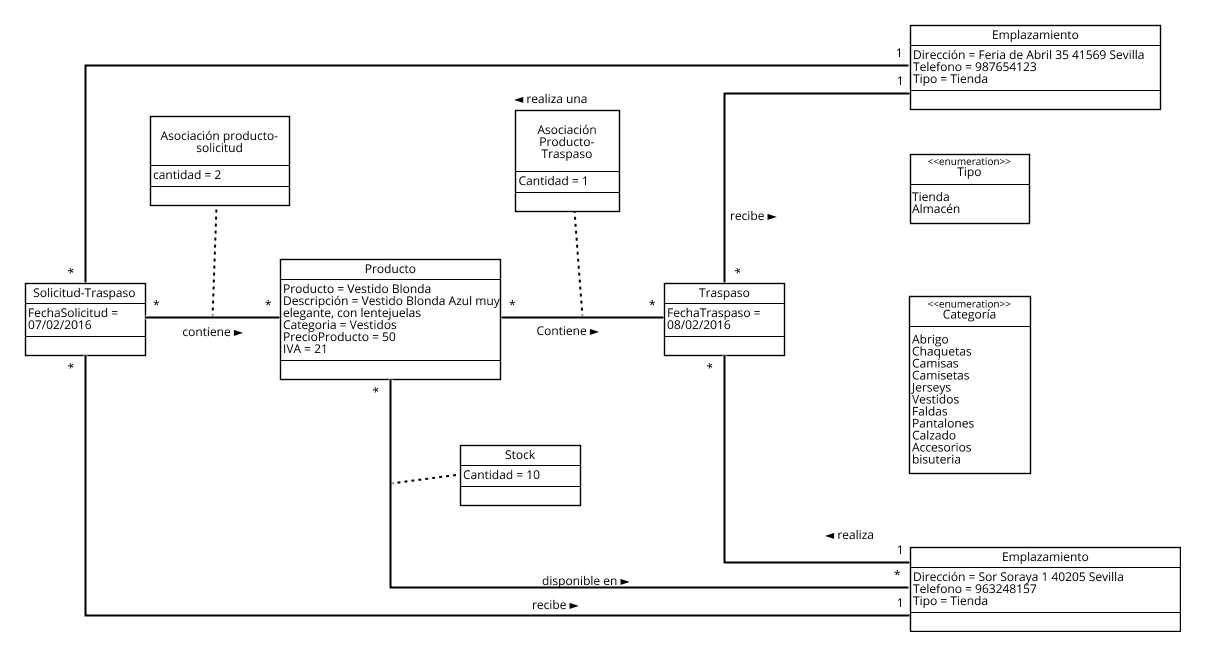
\includegraphics[width=\linewidth]{images/pruebas/traspaso-tienda-tienda.png}
	\caption{UML Traspaso Tienda - Tienda}
\end{figure}

\begin{figure}[H]
	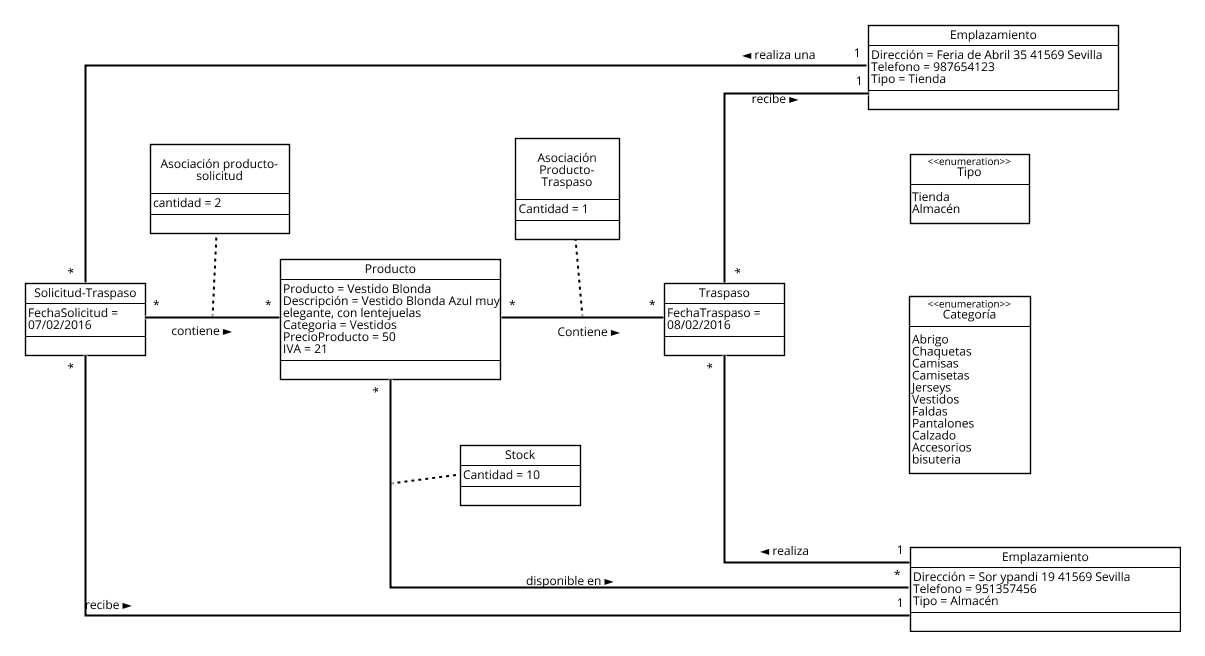
\includegraphics[width=\linewidth]{images/pruebas/traspaso-tienda-almacen.png}
	\caption{UML Traspaso Tienda - Almacén}
\end{figure}

\begin{figure}[H]
	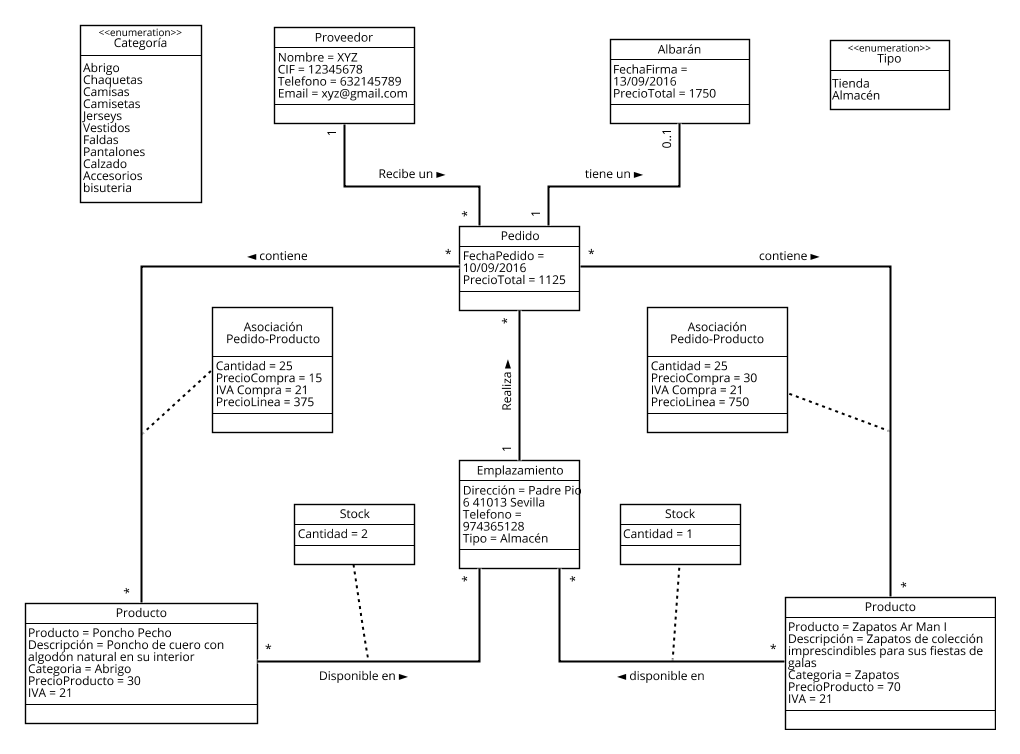
\includegraphics[width=\linewidth]{images/pruebas/pedido-tienda-proveedor.png}
	\caption{UML Pedido Tienda - Proveedor}
\end{figure}

\begin{figure}[H]
	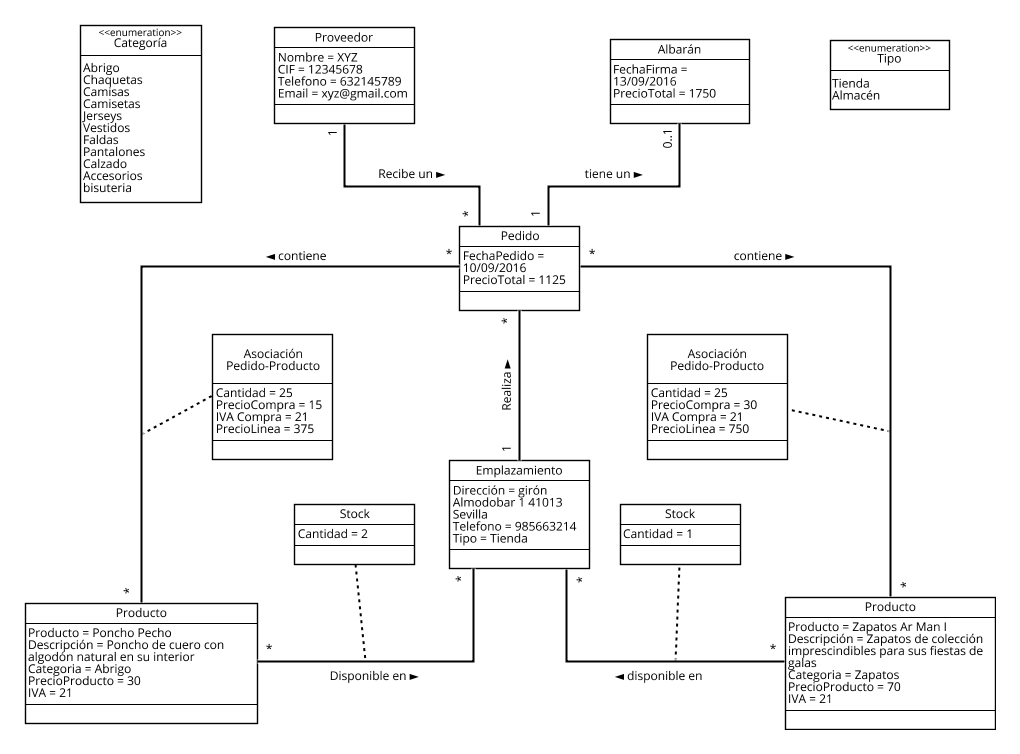
\includegraphics[width=\linewidth]{images/pruebas/pedido-almacen-proveedor.png}
	\caption{UML Pedido Almacén - Proveedor}
\end{figure}

\section{Matrices de trazabilidad}

\subsection{Pruebas de aceptación frente a requisitos}

\begin{table}[H]
	\centering
	\caption{\textbf{Requisitos funcionales}}
	\label{Requisitos funcionales}
	\resizebox{\textwidth}{!}{\begin{tabular}{|c|c|c|c|c|c|c|c|c|c|c|c|c|c|c|c|c|c|c|}
			\hline
			\textbf{PA-01} & x           &             &             &             &             &             &             &             &             &             &             &             &             &             &             &             &             &             \\ \hline
			\textbf{PA-02} &             &             &             &             &             &             &             &             &             &             &             &             &             &             &             &             & x           &             \\ \hline
			\textbf{PA-03} &             &             & x           & x           & x           &             &             &             &             &             &             &             &             &             &             &             &             &             \\ \hline
			\textbf{PA-04} &             &             &             &             &             & x           &             &             &             &             &             &             &             &             &             &             &             &             \\ \hline
			\textbf{PA-05} &             & x           &             &             &             &             & x           &             &             & x           &             &             & x           &             &             &             &             &             \\ \hline
			\textbf{PA-06} &             &             &             &             &             &             &             & x           &             &             &             &             &             &             &             &             &             &             \\ \hline
			\textbf{PA-07} &             &             &             &             &             &             &             &             & x           & x           &             &             &             &             &             &             &             & x           \\ \hline
			\textbf{PA-08} &             &             &             &             &             &             &             &             &             &             & x           & x           &             & x           &             &             &             &             \\ \hline
			\textbf{PA-09} &             &             &             &             &             &             & x           &             &             &             &             &             &             &             & x           & x           &             &             \\ \hline
			\textbf{PA-10} &             &             &             &             &             &             &             &             &             &             &             &             &             &             &             &             &             &             \\ \hline
			\textbf{PA-11} &             &             &             &             &             &             &             &             &             &             &             &             &             &             &             &             &             &             \\ \hline
			\textbf{}      & \textbf{01} & \textbf{02} & \textbf{03} & \textbf{04} & \textbf{05} & \textbf{06} & \textbf{07} & \textbf{08} & \textbf{09} & \textbf{10} & \textbf{11} & \textbf{12} & \textbf{13} & \textbf{14} & \textbf{15} & \textbf{16} & \textbf{17} & \textbf{18} \\ \hline
	\end{tabular}}
\end{table}

\begin{table}[H]
	\centering
	\caption{\textbf{Requisitos de informacion}}
	\label{Requisitos de informacion}
	\resizebox{\textwidth}{!}{\begin{tabular}{|c|c|c|c|c|c|c|c|c|c|c|c|}
			\hline
			\textbf{PA-01} & x           &             &             &             &             &             &             &             &             &             &             \\ \hline
			\textbf{PA-02} &             & x           &             &             &             &             &             &             &             &             &             \\ \hline
			\textbf{PA-03} &             &             & x           &             &             &             &             &             &             &             &             \\ \hline
			\textbf{PA-04} &             &             &             & x           &             &             &             &             &             &             &             \\ \hline
			\textbf{PA-05} &             &             &             &             & x           &             &             &             &             &             &             \\ \hline
			\textbf{PA-06} &             &             &             &             &             &             & x           &             &             &             &             \\ \hline
			\textbf{PA-07} &             &             &             &             &             &             &             & x           &             & x           &             \\ \hline
			\textbf{PA-08} &             &             &             &             &             &             &             &             & x           &             & x           \\ \hline
			\textbf{PA-09} &             &             &             &             &             & x           &             &             &             &             &             \\ \hline
			\textbf{PA-10} &             &             &             &             &             &             &             &             &             &             &             \\ \hline
			\textbf{PA-11} &             &             &             &             &             &             &             &             &             &             &             \\ \hline
			\textbf{}      & \textbf{01} & \textbf{02} & \textbf{03} & \textbf{04} & \textbf{05} & \textbf{06} & \textbf{07} & \textbf{08} & \textbf{09} & \textbf{10} & \textbf{11} \\ \hline
	\end{tabular}}
\end{table}

\begin{table}[H]
	\centering
	\caption{\textbf{Reglas de negocio}}
	\label{Reglas de negocio}
	\begin{tabular}{|c|c|c|c|c|c|}
		\hline
		\textbf{PA-01} &             &             &             &             & x           \\ \hline
		\textbf{PA-02} & x           &             &             & x           &             \\ \hline
		\textbf{PA-03} & x           &             &             &             &             \\ \hline
		\textbf{PA-04} &             & x           &             & x           &             \\ \hline
		\textbf{PA-05} &             &             & x           &             & x           \\ \hline
		\textbf{PA-06} &             & x           &             &             &             \\ \hline
		\textbf{PA-07} &             & x           &             &             & x           \\ \hline
		\textbf{PA-08} &             &             & x           &             &             \\ \hline
		\textbf{PA-09} &             &             & x           & x           &             \\ \hline
		\textbf{PA-10} & x           &             &             &             &             \\ \hline
		\textbf{PA-11} &             & x           &             &             &             \\ \hline
		\textbf{}      & \textbf{01} & \textbf{02} & \textbf{03} & \textbf{04} & \textbf{05} \\ \hline
	\end{tabular}
\end{table}

\subsection{Pruebas de aceptación frente a escenarios de prueba}

\begin{table}[H]
	\centering
	\caption{\textbf{Escenarios}}
	\label{Escenarios}
	\begin{tabular}{|c|c|c|c|c|c|c|c|c|c|c|c|}
		\hline
		\textbf{Escenario 01} &             &             &             & X           &             & X           & X           &             & X           &             & X           \\ \hline
		\textbf{Escenario 02} &             &             &             & X           &             & X           & X           &             & X           &             & X           \\ \hline
		\textbf{Escenario 03} &             &             &             & X           & X           &             &             & X           & X           &             &             \\ \hline
		\textbf{Escenario 04} &             &             &             & X           & X           &             &             & X           & X           &             &             \\ \hline
		\textbf{Escenario 05} & X           & X           &             & X           & X           &             &             &             &             &             &             \\ \hline
		\textbf{Escenario 06} & X           & X           & X           & X           & X           &             &             &             &             & X           &             \\ \hline
		\textbf{}             & \textbf{01} & \textbf{02} & \textbf{03} & \textbf{04} & \textbf{05} & \textbf{06} & \textbf{07} & \textbf{08} & \textbf{09} & \textbf{10} & \textbf{11} \\ \hline
	\end{tabular}
\end{table}

\subsection{Tipos de UML frente a Requisitos}

\begin{table}[H]
	\centering
	\caption{\textbf{Requisitos de informacion}}
	\resizebox{\textwidth}{!}{\begin{tabular}{|c|l|l|l|l|l|l|l|l|l|l|l|}
		\hline
		\textbf{Venta}             & x                                & x                                & x                                & x                                & x                                & x                                &                                  &                                  &                                  &                                  &                                  \\ \hline
		\textbf{Traspaso - Pedido} &                                  &                                  &                                  & x                                & x                                & x                                & x                                & x                                & x                                & x                                & x                                \\ \hline
		\textbf{}                  & \multicolumn{1}{c|}{\textbf{01}} & \multicolumn{1}{c|}{\textbf{02}} & \multicolumn{1}{c|}{\textbf{03}} & \multicolumn{1}{c|}{\textbf{04}} & \multicolumn{1}{c|}{\textbf{05}} & \multicolumn{1}{c|}{\textbf{06}} & \multicolumn{1}{c|}{\textbf{07}} & \multicolumn{1}{c|}{\textbf{08}} & \multicolumn{1}{c|}{\textbf{09}} & \multicolumn{1}{c|}{\textbf{10}} & \multicolumn{1}{c|}{\textbf{11}} \\ \hline
	\end{tabular}}
\end{table}

\begin{table}[H]
	\centering
	\caption{\textbf{Reglas de negocio}}
	\begin{tabular}{|c|c|c|c|c|c|}
		\hline
		\textbf{Venta}             & x           &             &             & x           & x           \\ \hline
		\textbf{Traspaso - Pedido} &             & x           & x           &             & x           \\ \hline
		\textbf{}                  & \textbf{01} & \textbf{02} & \textbf{03} & \textbf{04} & \textbf{05} \\ \hline
	\end{tabular}
\end{table}

\begin{table}[H]
	\centering
	\caption{\textbf{Requisitos Funcionales}}
	\resizebox{\textwidth}{!}{\begin{tabular}{|c|c|c|c|c|c|c|c|c|c|c|c|c|c|c|c|c|c|c|}
		\hline
		\textbf{Venta}            & X           & X           & X           & X           & X           & X           & X           &             &             &             &             &             &             &             & X           & X           & X           &             \\ \hline
		\textbf{Traspaso - Venta} &             &             &             &             &             & X           & X           & X           & X           & X           & X           & X           & X           & X           & X           & X           &             & X           \\ \hline
		\textbf{}                 & \textbf{01} & \textbf{02} & \textbf{03} & \textbf{04} & \textbf{05} & \textbf{06} & \textbf{07} & \textbf{08} & \textbf{09} & \textbf{10} & \textbf{11} & \textbf{12} & \textbf{13} & \textbf{14} & \textbf{15} & \textbf{16} & \textbf{17} & \textbf{18} \\ \hline
	\end{tabular}}
\end{table}

\section{Modelos relacionales}
Para poder pasar de UML(MC) a 3FN(MR), tenemos que ser capaces de normalizar tanto en 2FN como en 1FN,
esto lo hemos comprobado de la siguiente manera:
En cada tupla de la 3FN se le asigna a cada atributo un solo valor del dominio sobre el que está definido, es decir, no existen atributos con
varios valores. Esto prueba que está en 1FN.
Tras asegurar la 1FN, pasamos a la comprobación de la 2FN, para validar esta normalización tenemos que tener en cuenta que los atributos que no
sean Primary Key o Foreign Key (atributos no primos) deben de ser dependientes de estas claves, esto lo cumplimos gracias a las foreign keys y
primary keys creadas para las asociaciones, esta relación está explicada más adelante.
Finalmente llegamos a la comprobación de la 3FN, para esta comprobación tenemos que tener en cuenta que la relación tiene que estar en 2FN y que
la relación de tablas simplemente se haga mediante las primary y las foreign key, todo lo que no sea claves candidatas no puede estar en
varias entidades asociadas a la vez.

\subsection{3FN Venta}

 \begin{itemize}
 	\item[Socio] Los atributos son directos en la 3FN, añadiendo que DNI será una primray key. Tiene una relación 0..1 - n con Venta, venta mantiene todos sus atributos de manera directa en la 3FN, añadiendo un ID\_VENTA como
primary key y debido a la relación con socio una foreign key llamada DNI.
 	\item[Venta] Tiene una relación n - m con Producto, se crea una tabla intermedia debido a esta relación que es la tabla VentaProducto, con los siguientes
atributos: cantidad, precioVenta e ivaVenta. Además tiene ID\_VENTA y ID\_PRODUCTO como primary keys y foreigns keys, estas claves son provocadas
por la relación n - m entre Venta y Producto.
 	\item[Producto] La tabla producto mantiene todos sus atributos de manera directa  en la 3FN y añade ID\_PRODUCTO que será su primary key.
 	\item[Venta] Tiene una relación 1 - 1 con Factura, factura mantiene todos sus atributos de manera directa  en la 3FN y añade un ID\_FACTURA como primary key, un ID\_VENTA
 	como foreign key debido a la relación con Venta y un ID\_EMPLAZAMIENTO debido a la relación con Emplazamiento.
 	\item[Factura] tiene una relación n - 1 con Emplazamiento, emplazamiento  mantiene todos sus atributos de manera directa en la 3FN y añade un ID\_EMPLAZAMIENTO como
 	primary key.
 	\item[Producto] Tiene una relación n - m con Emplazamiento, esto da lugar a la creación de una tabla intermedia, para poder tratar la relación n - m, con
 	los siguientes atributos: cantidad, ID\_PRODUCTO(primary key y foreign key) y ID\_EMPLAZAMIENTO(primary key y foreign key). Estas claves son provocadas por
 	la relacion n - m entre Producto y Emplazamiento.
 	
 \end{itemize}

\begin{figure}[H]
	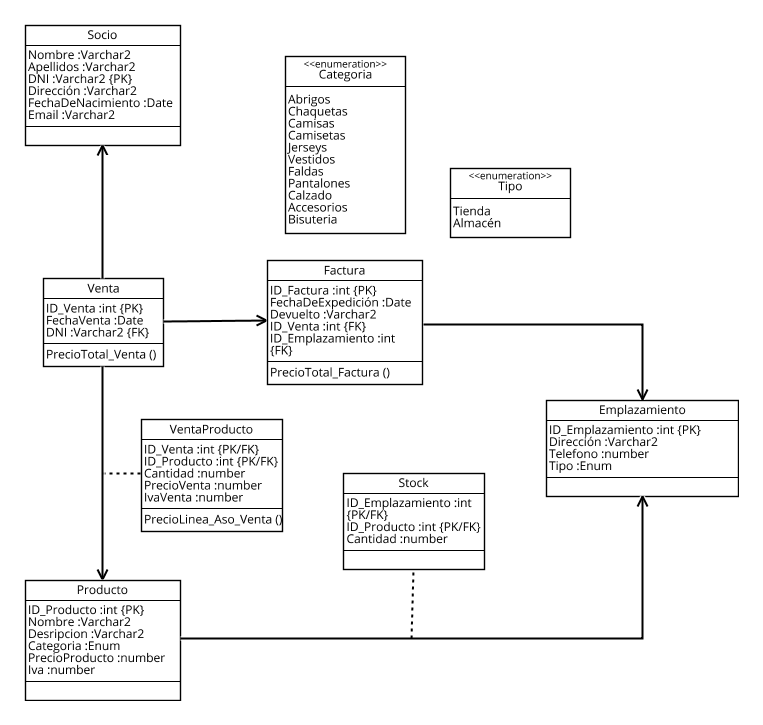
\includegraphics[width=\linewidth]{images/3FN/3FN-venta.png}
	\caption{3FN Venta}
\end{figure}

\subsection{3FN Traspaso - Pedido}

\begin{itemize}
	\item [Proveedor] Tiene una relación 1 - n con Pedido, proveedor mantiene todos sus atributos de manera directa en la 3FN y añade un ID\_PROVEEDOR como primary key.
	\item [Emplazamiento] Tiene una relación 1 - n con Pedido, pedido mantiene todos sus atributos de manera directa  en la 3FN, añade un ID\_PEDIDO como primary key y un
	ID\_PROVEEDOR como foreign key debido a la relación con Proveedor.
	\item [Pedido] Tiene una relación n - m con Producto, se crea una tabla intermedia debido a esta relación que es la tabla Asociación Pedido-Producto, con los
	siguientes atributos: cantidad, precioCompra, ivaCompra. Además tiene ID\_PEDIDO y ID\_PRODUCTO como primary keys y foreigns keys, estas claves son provocadas
	por la relación n - m entre Pedido y Producto.
	\item[Albarán] Tiene una relación 1 - 0..1 con Pedido, albarán mantiene todos sus atributos de manera directa en la 3FN y añade un ID\_ALBARAN como primary key.
	\item[Emplazamiento] Tiene una relación 1 - m bidireccional con Traspaso, traspaso mantiene todos sus atributos de manera directa en la 3FN y añade un ID\_TRASPASO.
	
	\item[Emplazamiento] Tiene una relación 1 - m bidireccional con Solicitud-Trapaso, solicitud-traspaso mantiene todos sus atributos de manera directa en la 3FN
	y añade un ID\_Solicitud.
	\item[Traspaso] Tiene una relación n - m con Producto, esto da lugar a la creación de una tabla intermedia, para poder tratas la relación n-m, con los siguientes
	atributos: cantidad, ID\_Producto(primary key y foreign key) y ID\_Traspaso(primary key y foreign key). Estas claves son provocadas por la relación n - m
	entre Traspaso y Producto.
	\item[Solicitud-Trapaso] Tiene una relación n - m con Producto, esto da lugar a la creación de una tabla intermedia, para poder tratas la relación n-m, con los siguientes
	atributos: cantidad, ID\_Producto(primary key y foreign key) y ID\_SOLICITUD(primary key y foreign key). Estas claves son provocadas por la relación n - m
	entre Solicitud-Traspaso y Producto.
	
\end{itemize}

\begin{figure}[H]
	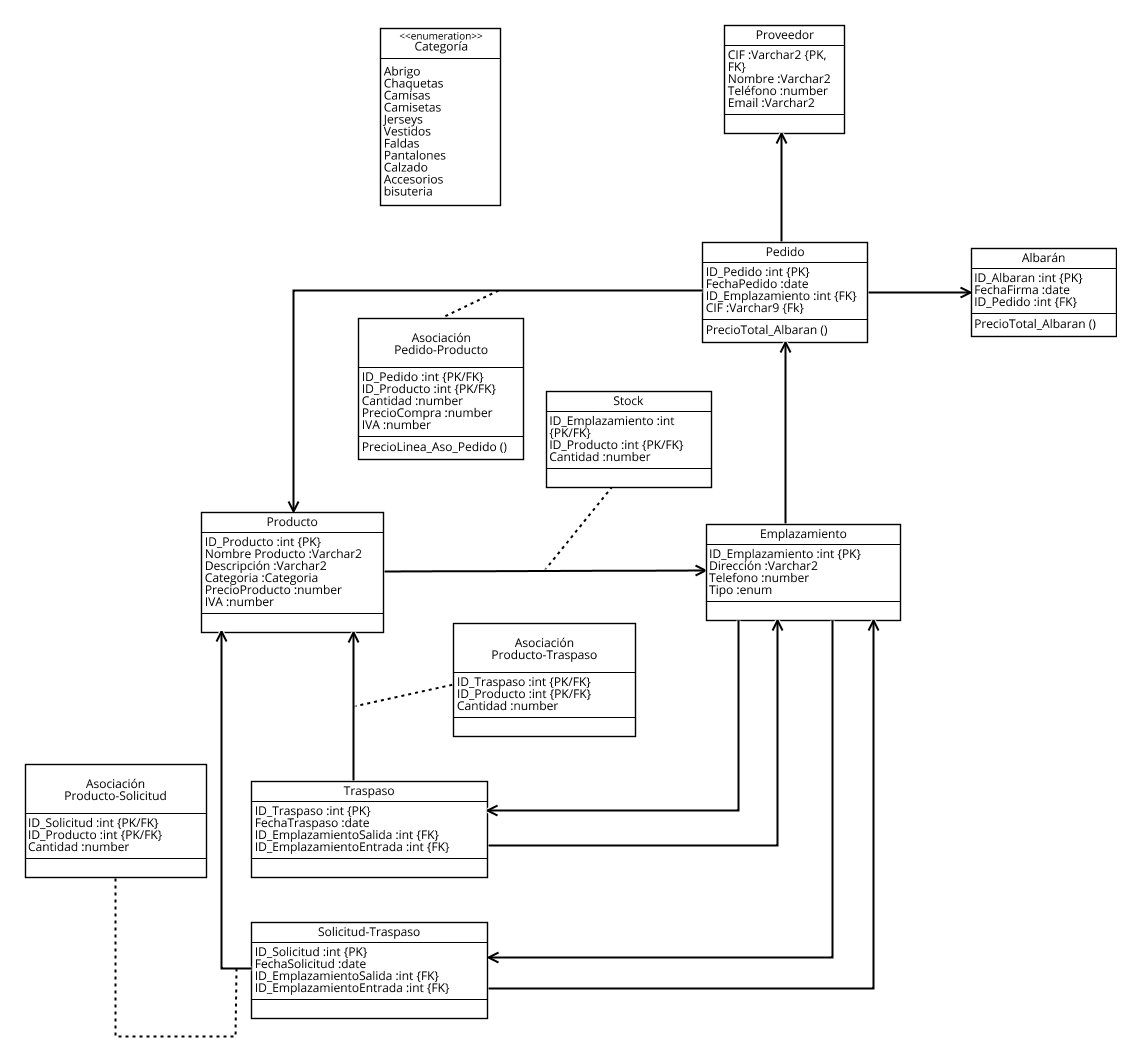
\includegraphics[width=\linewidth]{images/3FN/3FN-traspaso-pedido.png}
	\caption{3FN Traspaso - Pedido}
\end{figure}

\section{Código SQL de la base de datos}

\subsection{Tablas}
\lstinputlisting[language=SQL]{sql/tablas.sql}<

\subsection{Funciones y Procedures}
\lstinputlisting[language=SQL]{sql/funciones_y_procedures.sql}

\subsection{Triggers}

\lstinputlisting[language=SQL]{sql/triggers.sql}

\subsection{Pruebas}
\lstinputlisting[language=SQL]{sql/pruebas.sql}

\section{Apéndice}
\subsection{Actas de reunión}

\includegraphics[height=16cm, center]{images/acta1.jpg} \newpage

\includegraphics[height=16cm, center]{images/acta2.jpg}
\end{document}